%%%%%%%%%%%%%%%%%%%%%%%%%%%%%%%%%%%%%%%%%
% University Assignment Title Page 
% LaTeX Template
% Version 1.0 (27/12/12)
%
% This template has been downloaded from:
% http://www.LaTeXTemplates.com
%
% Original author:
% WikiBooks (http://en.wikibooks.org/wiki/LaTeX/Title_Creation)
%
% License:
% CC BY-NC-SA 3.0 (http://creativecommons.org/licenses/by-nc-sa/3.0/)
% 
% Modified for COSC480/490 by: Louis Whitburn
% Lech Szymanski (8/3/18)

\documentclass[12pt]{article}
\usepackage[draft]{cosc4x0style}

\usepackage{listings}

\usepackage{biblatex}

\usepackage{xcolor}

% Encoding goodness that I usually expect to rely on...
\usepackage[T1]{fontenc}
\usepackage[utf8]{inputenc}

\definecolor{codegreen}{rgb}{0,0.6,0}
\definecolor{codegray}{rgb}{0.5,0.5,0.5}
\definecolor{codepurple}{rgb}{0.58,0,0.82}
\definecolor{backcolour}{rgb}{0.95,0.95,0.92}

\lstset{
	backgroundcolor=\color{backcolour},   
	commentstyle=\color{codegreen},
	keywordstyle=\color{blue},
	numberstyle=\color{codegray},
	stringstyle=\color{codepurple},
	breaklines=true,
	breakatwhitespace=true,
	numbers=left,
	basicstyle=\ttfamily\small
}
 
\usepackage{amssymb}
\usepackage{amsmath}

\usepackage{graphicx}

\usepackage{wrapfig}

\addbibresource{bibliography.bib}

% The sorts of macros that I (Dave) normally use when working with LaTeX
\newcommand{\note}[2][red]{\textcolor{#1}{#2}}
\newcommand{\notedme}[1]{\note[blue]{[<Dave> #1]}}
\newenvironment{scaffold}{\color{red}}{}
\newcommand{\change}[2][]{\textcolor{orange}{#2}}

% To compile the final version of the report (which will remove all the todo content)
%\usepackage{cosc4x0style}

% Specify project code 480 or 490
\papercode{490}

% Your project title
\title{Kalman Filtering in Verilog}

% Your name
\author{Louis \textsc{Whitburn}}
\studentid{2548261}

% Names of your supervisors, separated by line break '\\'
\supervisors{
	Dr.\@ David \textsc{Eyers} \\
  	Dr.\@ Tim \textsc{Molteno}
}

% Date, change the \today to a set date if you want to be precise
\reportdate{\today}

\begin{document}


\maketitle

\begin{abstract}

With the surge in growth of the UAV (unmanned aerial vehicle) and the smartphone industry, there continues to be significant demand for accurate and low power methods to measure and estimate physical orientation. The simplest method of estimating a device's orientation is by comparing the device's orientation to gravity, i.e.\@ by using accelerometers. This method is very easy to implement, however it becomes very inaccurate when the device is actually accelerating. To improve accuracy while the device is accelerating we can combine measurements from multiple sensors---such as gyroscopes and magnetometers---to calculate a more accurate estimate. This process is called ``sensor fusion'', and one of the most well known methods for performing sensor fusion is the Kalman filter. Unfortunately, the Kalman filter requires some fairly computationally expensive matrix mathematics, which limits potential performance, and results in greater than necessary power drain when implemented in software. These existing software implementations are usually sufficient for their specific applications, however improving performance is always beneficial, and lowering power consumption is very important in devices that require recharging, such as smartphones. My project explores implementing the required matrix mathematics for the Kalman filter in hardware, the tradeoffs between hardware resource consumption and performance, and how the choices of numeric representation affect the accuracy of the inferred orientation. This last point is of particular importance given that hardware is extremely flexible with how numbers can be represented. 

\end{abstract}

\section{Introduction}

Physical orientation estimation is critical in devices such as smartphones, be it for improving the accuracy of GPS measurements, or for features such as automatically switching the display between landscape and portrait. While the sales of smartphones have slowed down in recent years, the industry is still very strong, with over one billion units sold per year \cite{Mongardini_2020} over the last few years. In addition, the smartphone market is not the only industry that requires accurate orientation estimation---it is even more critical in systems such as augmented / virtual reality devices or unmanned aerial vehicles (UAVs).

Orientation estimation is an application of state estimation, where the state we want to estimate is orientation. State estimation is the process of using multiple measurements to provide an estimate of the state of a system. This is particularly important in control systems where having better knowledge of the current state of the system makes it easier to control. The Kalman filter is still considered the ``go-to'' approach for solving state estimation problems due to its simplicity and good performance. The main downside of the Kalman filter is that many implementations continue to be mostly software based~\cite{ayub_2012}. This isn't ideal from an efficiency standpoint since software implementations---while being very flexible---are not particular power efficient or fast. This is simply because modern CPUs can only run one instruction at a time, per core or pipeline. Most of the advancements in modern CPU performance have been about getting around that limit in one of two ways:
\begin{itemize}
	\item Improving how fast individual instructions can run, e.g.\@ by increasing the clock speed, reducing the number of clock cycles it takes to execute an instruction on average (e.g.\@ caching making subsequent memory read instructions faster), or with technologies such as simultaneous multithreading (SMT), SIMD instructions (such as AVX) and branch prediction\footnote{Which turned out to cause more problems than it solved with bugs such as Meltdown and Spectre. \notedme{Speculative exectuion and branch prediction are not equivalent. You can have branch prediction strategies without speculative execution.} }.
	\item Making CPUs more parallel, such as by adding more CPU cores per CPU, or by having motherboards that have multiple CPU sockets.
\end{itemize}
These technologies improve performance, however they introduce complexity into the CPU architectures, contributing to greater power use\footnote{There is a subtlety here---since they allow instructions to execute faster they result in lower power usage per instruction, however they increase energy use per unit of time.}. In addition, there is a limit, in terms of power, heat dissipation, and physical space to how many cores that can fit in a CPU. Because of this, it is quite common to implement some functions in dedicated hardware, such as using graphics processing units (GPUs) for rendering as opposed to software rendering.

Several hardware-based Kalman filter implementations have been developed, however they are either too complex \cite{mills_2016} to be synthesised to a cheap field programmable gate array (FPGA), or are encumbered with intellectual property restrictions\footnote{Such as this one from Altera: \url{https://www.intel.com/content/dam/www/programmable/us/en/pdfs/literature/ds/extended_kalman_filter.pdf}}. I aim to produce a design that can be synthesised to any reasonably-sized FPGA which could then be interfaced with sensors to give an estimate of orientation.

I want to target an FPGA because they are available, inexpensive, and are considered to be ``real hardware'', as opposed to just running my hardware in a simulator. An FPGA is a silicon chip which consists of a large quantity of lookup tables (LUTs), and a switching fabric which connects the LUTs. FPGAs are ``field programmable'', i.e.\@ they can be reconfigured. In particular, the LUTs act like reprogrammable logic gates, and the switching fabric is reconfigurable allowing different LUTs to be joined together in different ways. This means that it is very easy to test and develop hardware on an FPGA, which allows the expensive and time consuming fabrication process to be delayed until it is time to start manufacturing the final hardware design.

The primary motivation behind moving from a software implementation to a hardware implementation is reduced power consumption, although there will be an increase in performance as well. Most software Kalman filter implementations are already ``good enough'', i.e.\@ the reported data is sufficiently accurate for their application's target domain, however there is always the potential to do better, in terms of precision of the output data, or the frequency in which the state estimate is updated. In addition, an increase in performance could be used to justify lowering the data input frequency, which would further lower power consumption. Moving the Kalman filter to hardware would also increase flexibility, allowing the CPU cycles that were used running the Kalman filter in software to do other work.

\section{Background}

I would like to start by introducing inertial measurement units (IMUs) and their theoretical background: Sequential inference and the Kalman filter. I will also discuss the different algorithmic approaches for implementing the matrix operations required for the Kalman filter. I would then like to discuss Hardware Description Languages (HDLs), and comment on the typical differences between software and hardware solutions to problems in order to give some context for why hardware implementations tend to perform better than software implementations.

\subsection{Inertial Measurement Units}

An IMU is a device that provides orientation (and occasionally position) estimations. As I have already discussed, these orientation estimations are often provided by the Kalman filter, and the theoretical basis for the Kalman filter---sequential inference---is discussed below.

\subsubsection{Sequential Inference}

Sequential inference \cite{morrison_2016} is the process of repeatedly adding information to a model of a system to improve our understanding of the state that system is in. In particular, we can derive
\begin{equation}
	\label{si}
	P(S | D_k, m) = {P(D_k | S, m) P(S | m) \over P(D_k | m)}\,,
\end{equation}
where $S$ is the state, $D_k$ are the measurements at time step $k$, and $m$ is the model. What this equation is saying is that probability of the system being in some state, given some measurements and a model, is equal to the product of the probability of making some measurement, given the state and the model, weighted by the ratio between the probability of being in that state (given a model of the system) and the probability of making those measurements (given a model of the system). This is simply an application of Bayes' Theorem:
\begin{equation}
	P(A | B) = {P(B|A) P(A) \over P(B)}
\end{equation}
The significance of being based off of Bayes's Theorem is that it means that equation \ref{si} can be composed to give:
\begin{equation}
	P(S|D_{k+1},D_k,m) = {P(D_{k+1}|D_k,S,m) \over P(D_{k+1}|D_k,m)} P(S | D_k, m)
\end{equation}
Thus we can add more measurements to our system to gain a better understanding of the state that it is in. Sequential inference provides the theoretical basis for the Kalman Filter, which is one of the most widely used applications of sequential inference.

\subsubsection{Kalman Filter}

The Kalman filter \cite{kalman_1960} is one of the most popular solutions for estimating the state (e.g.\@ orientation) of a system from multiple noisy sensors, due to its relative simplicity while still performing optimally\footnote{Here, optimally refers to how the calculated ``Kalman gain'' minimises the ``\emph{a posteriori} residual'', which is discussed later in this section.} \cite{wangyan_2015}. It works by using a model of the system to predict the future state of that system, and then (after some time step), comparing that predicted state to the measured state.

The first two steps are to predict how the system will evolve:
\begin{eqnarray}
	\mathbf{\hat{x}}_{k | k-1} &=& \mathbf{F}_k \mathbf{\hat{x}}_{k-1|k-1} + \mathbf{B}_k \mathbf{u}_k\\
	\mathbf{P}_{k|k-1} &=& \mathbf{F}_k \mathbf{P}_{k-1 | k-1} \mathbf{F}^T_k + \mathbf{Q}_k
\end{eqnarray}
Here, $\mathbf{\hat{x}}_{k | k-1}$ and $\mathbf{P}_{k|k-1}$ are the \emph{a priori} (i.e.\@ without including any additional knowledge) estimates of the state, and the covariance of the state. Our \emph{a priori} knowledge comes only from the previous state---the $k-1|k-1$ subscripts. $\mathbf{F}_k$ is the state transition matrix, i.e.\@ it determines how the state changes through time. $\mathbf{B}_k$ is the control-input matrix applied to the control vector $\mathbf{u}_k$---these model any external input to the system, i.e.\@ if it was forced in some direction. Finally, $\mathbf{Q}_k$ is the covariance of the process noise, i.e.\@ the error / uncertainty that arises from the model. This uncertainty mainly arises from approximations made in the model (e.g.\@ linearisation), and from integration error (e.g.\@ if the measurement is velocity, then the estimate of position will drift if not corrected).

The next step is the update step. It first consists of the innovation stage---determining the difference between the predicted / forecast state and the observed state:
\begin{eqnarray}
	\mathbf{\tilde{y}}_k &=& \mathbf{z}_k - \mathbf{H}_k \mathbf{\hat{x}}_{k|k-1} \\
	\mathbf{S}_k &=& \mathbf{H}_k \mathbf{P}_{k|k-1} \mathbf{H}^T_k + \mathbf{R}_k 
\end{eqnarray}
Here $\mathbf{\tilde{y}}_k$ is that difference (residual), where $\mathbf{z}_k$ is the measured state and $\mathbf{\hat{x}}_{k|k-1}$ is the \emph{a priori} estimate from before. $\mathbf{H}_k$ is the observation model, which maps the state space into the observation space---e.g.\@ when measuring depth via sonar the state space contains the depth, whereas the measured state contains the sonar round trip time. The observation model converts this (predicted) state into a (predicted) observation, in this case by dividing the distance by half the speed of sound in water. $\mathbf{S}_k$ is the residual of the covariance, where $\mathbf{R}_k$ is the covariance of the process noise, in the above example, this could arise from water currents and temperature differences slightly affecting the speed of sound in the water. It could also arise from imprecise sensors.

The second part of the update step is determining the Kalman gain:
\begin{eqnarray}
	\mathbf{K}_k = \mathbf{P}_{k|k-1} \mathbf{H}^T_k \mathbf{S}^{-1}_k
\end{eqnarray}
This generates a gain matrix which aims to minimise the \emph{a posteriori} (updated with the sensor observations) residual, $\mathbf{\tilde{y}}_{k|k} = \mathbf{z}_k - \mathbf{H}_k \mathbf{\hat{x}}_{k|k}$.

The final part is generating these \emph{a posteriori} estimates:
\begin{eqnarray}
	\mathbf{\hat{x}}_{k|k} &=& \mathbf{\hat{x}}_{k|k-1} + \mathbf{K}_k \mathbf{\tilde{y}}_k \\
	\mathbf{P}_{k|k} &=& (\mathbf{I} - \mathbf{K}_k \mathbf{H}_k)\mathbf{P}_{k|k-1}
\end{eqnarray}
Here $\mathbf{\hat{x}}_{k|k}$ and $\mathbf{P}_{k|k}$ are the \emph{a posteriori} state estimate and state estimate covariance.

Thus we have a mechanism to have our estimate of the state optimally track the actual state. In the above equations, the matrices (uppercase and bold) are of the size $n \times n$ and the vectors (lowercase and bold) are column vectors of the size $n \times 1$, where $n$ is the size of the estimated state. The observation space need not be the same size as the state space, thus if the size of the observation space is $m$, then $\mathbf{H}_k$ may be $m \times n$ and $\mathbf{z}_k$ may be $m \times 1$. Going forward I will assume that $n = m$ for simplicity, since if, for example, the state space is larger than the observation space, then we can simply expand the observation space matrices and vectors with zeros to bring them up to the correctly sized (square) matrices or vectors.

\subsection{Naive Matrix Algorithms}
\label{naive}

For this project, the required matrix operations are:

\begin{itemize}
	\item Addition and subtraction
	\item Multiplication (by a vector or other matrix)
	\item Scaling (multiplication by a scalar)
	\item Transposition
	\item Calculation of the determinant
	\item Inversion
\end{itemize}

Of these, transposition is by far the easiest since it is nothing more than shuffling some data around. The next easiest are addition and subtraction, since they just involve adding or subtracting some numbers. This requires some care when it comes to numeric overflow and optimisation, but this is not too difficult. The next easiest is scaling, which can be implemented by something as simple as a loop through all of the elements of the vector or matrix, multiplying each element by the scaling factor. Multiplication by a vector or matrix is also comparatively simple, as it is just several \change{applications} of dot products.

The two more difficult operations are the determinant and inverse. The naive matrix determinant algorithm \cite{strang2006linear} is:
\begin{equation}
	\det{\mathbf{A}} = 
	\begin{cases}
	a_{11}a_{22} - a_{12}a_{21}& \mathbf{A} \in M_{2 \times 2}(\mathbb{R})\\
	\sum_{j=1}^{n} a_{1j}  (-1)^{j-1}\det{\mathbf{A}^{1j}} & \mathbf{A} \in M_{n \times n}(\mathbb{R}), n > 2\\
	\end{cases}
\end{equation}
Here $\mathbf{A}^{ij}$ means the matrix $\mathbf{A}$, but excluding row $i$ and column $j$. To give an estimate of complexity, a $4\times4$ matrix would require four $3\times3$ matrix determinants to be calculated, and each one of those would require three $2\times2$ matrix determinants to be calculated. Thus this is $\mathcal{O}(n!)$ (where $n$ is the amount of rows in the matrix), i.e.\@ very slow.

The inverse is even more complicated:
\begin{equation}
	a^{-1}_{ij} = \frac{1}{\det{\mathbf{A}}} \left((-1)^{i+j} \det{\mathbf{A}^{ij}}\right)^T
\end{equation}
Here $a^{-1}_{ij}$ is row $i$ and column $j$ of $\mathbf{A}^{-1}$. This is also $\mathcal{O}(n!)$, due to the $\frac{1}{\det{\mathbf{A}}}$ factor requiring an $n \times n$ determinant.

These are sufficient for small matrices, however for this project I am targeting a $12 \times 12$ matrix (three axes for each of orientation, angular velocity, acceleration and magnetic field strength). Thus, assuming a $2\times2$ matrix takes one time step, a $12 \times 12$ would take $\frac{12!}{2!} \approx 2.4 \times 10^8$ time steps. This is obviously unacceptable if we expect a Kalman Filter based off of this to operate in real time\footnote{Or in any reasonable time at all---a typical FPGA runs with a clock frequency on the order of 100 MHz, so if a $2\times2$ operation takes only one clock cycle it would still take a whole second to perform one matrix determinant calculation.}.

\subsection{Better Matrix Algorithms}
\label{lu}

\notedme{Make the first sentence self-contained: don't start with a sentence that continues the thread of the preceding paragraph when it's across a subsection boundary.}
Thankfully there are better ways\footnote{This is very common with numerical methods where often the more intuitive methods are mathematically ``cleaner'', however they tend to be slower or more numerically unstable than the less intuitive but more optimised algorithms. For example, the QR factorisation---which is briefly discussed later---decomposes a matrix into an orthogonal matrix $\mathbf{Q}$ and an upper triangular matrix $\mathbf{R}$. The usual process for orthogonalization is the Gram–Schmidt process, which projects vectors onto an orthonormal basis. Unfortunately the Gram–Schmidt process is numerically unstable so Householder reflections are often used instead, which are conceptually less intuitive.}. Imagine we had two special matrices: A lower triangular matrix $\mathbf{L}$, and an upper triangular matrix $\mathbf{U}$, both square matrices with size $n \times n$. Let's also imagine that the values on the diagonal of $\mathbf{L}$ are all 1. We can explore how these matrices have much better properties for finding the determinant and inverse of their product, $\mathbf{LU}$.

\subsubsection{Determinant}
Consider $\det(\mathbf{LU})$. We can simplify this by doing the following:
\begin{align}
	\det(\mathbf{LU}) &= \det(\mathbf{L}) \det(\mathbf{U}) \label{lu_det_1} \\
	&= \det(\mathbf{L}^T) \det(\mathbf{U}) \label{lu_det_2} \\
	&= \det(\mathbf{U}) \label{lu_det_3} \\
	&= \sum_{i=1}^{n} u_{ii} \label{lu_det_4}
\end{align}
Equations \ref{lu_det_1} and \ref{lu_det_2} are fairly straightforward, as they arise from the determinant of the product of two matrices being equal to the product of the determinants of those two matrices, and the determinant of any matrix being equal to the determinant of its transpose. Equations \ref{lu_det_3} and \ref{lu_det_4}
arise from the determinant of an upper triangular matrix being simply the product of its diagonal entries. The reason for this is that if---when calculating the determinant the naive way---we use the left column for the multiplication factors, as opposed to the top row\footnote{The same argument applies if we do use the top row, except that it applies to \emph{lower} triangular matrices. Since we can easily transpose a lower triangular matrix to form an upper triangular matrix I will only show the result for upper triangular matrices and just transpose $\mathbf{L}$ when needed.}, then we only need to calculate one minor, since all the rest will be multiplied by zero. Thus we only have to calculate one determinant for each iteration of the recursion, and multiply it by the value on the diagonal (the top left value). When we reach the base $2\times2$ case, the bottom left value will be zero, thus the determinant will be the product of the two diagonal elements. Thus as we work back from the bottom of the recursion we only ever multiply the values on the diagonal.

This means calculating the determinant of $\mathbf{LU}$ is $\mathcal{O}(n)$\cite{GoluVanl96}, which is a huge improvement over $\mathcal{O}(n!)$.

\subsubsection{Inverse}
Working out the inverse is also simple since we simply need to solve $\mathbf{LUx}=\mathbf{i}$ $n$ times, where $\mathbf{x}$ is the $n$\textsuperscript{th} column of $\mathbf{X}$ (which holds the inverse of $\mathbf{LU}$) and where $\mathbf{i}$ is the $n$\textsuperscript{th} column of $\mathbf{I}$ (the identity matrix). This is incredibly straightforward, since $\mathbf{L}$ and $\mathbf{U}$ are both triangular, thus we can use forward and back substitution to solve this as two sets of simultaneous equations.

This is $\mathcal{O}(n^3)$, since the forward and back substitution is quadratic in $n$, and we have to perform one for each column.

\subsubsection{LU Decomposition}
The above results are very promising, assuming we have these special matrices $\mathbf{L}$ and $\mathbf{U}$, however most matrices that we want to perform operations on don't come in that specific form. What we need is a process to factor some generic matrix $\mathbf{A}$ into $\mathbf{A}=\mathbf{LU}$.

This process is called the ``LU Decomposition''\cite{lu_decomposition}. It also provides a third matrix, $\mathbf{P}$, the permutation matrix. This is because the LU decomposition is based off of Gaussian elimination, which may require swapping rows, and thus to rebuild $\mathbf{A}$ from $\mathbf{L}$ and $\mathbf{U}$ we need to know which rows were swapped, thus $\mathbf{PA}$ = $\mathbf{LU}$. Since $\mathbf{P}$ only involves swapping rows, we were able to ignore it in the results above. The details of the LU decomposition are unimportant, beyond that it involves Gaussian elimination, however what is important to note is that the LU decomposition is $\mathcal{O}(n^3)$. Since the inversion or determinant steps come after the LU decomposition, the complexity is added, not multiplied. Thus calculating the determinant and inverse is still only $\mathcal{O}(n^3)$ i.e.\@ polynomial.

One corollary of the above is this: We can still implement the naive inverse using the better determinant. Since the naive inverse requires $n^2$ determinants (of size $n-1 \times n-1$, which is still $\mathcal{O}(n^3)$), this means that this ``semi-naive'' approach is $\mathcal{O}(n^5)$. This is still significantly better than $\mathcal{O}(n!)$, and I will discuss this aspect more later in this report.

In addition to the LU decomposition there is also the QR decomposition, and the singular value decomposition (SVD)~\cite{num_lin_alg}, among others. The QR decomposition was not chosen because it is slightly slower that the LU decomposition (about twice as slow), and the SVD was not chosen because it is harder to implement, and because it is more suited to solving homogenous equations, which are those of the form $\mathbf{A}\mathbf{x}=\mathbf{0}$. Alternatively, if there is no such $\mathbf{x}$ that satisfies $\mathbf{A}\mathbf{x}=\mathbf{0}$, then it can also be used to solve the ``least-squares'' problem, where we want to find the $\mathbf{x}$ which minimises $||\mathbf{Ax}||_2$ (the 2-norm of $\mathbf{Ax}$---for a vector this will be the magnitude). This is extremely important (and with the SVD, very fast), however this is not relevant to this project.

\subsection{Hardware Description Languages}

The 1975 MOS Technology 6502 consists of approximately 3500 transistors. This is a comprehensible size, in that it is entirely possible to imagine it being designed by hand. On the other hand, the first CPU to introduce the x86 instruction set was the Intel 8086 back in 1978, made from some 29,000 transistors. An Intel Nehalem CPU from 12 years ago contains upwards of 750 million transistors. AMD's ``Epyc'' lineup of server CPUs contain up to 50 billion transistors per CPU. These would either be difficult and time consuming to design by hand (in the case of the 8086), or downright impossible to design by hand (the modern Nehalem and Epyc Rome CPUs). Thus it was the development of Hardware Description Languages (HDLs) that enabled us to make our huge modern integrated circuits in a reliable fashion.

If I write a program in a language such as C, and target a conventional architecture, such as ARM or x86, then the code that I write is not the actual program---it only describes the program. For example, no CPUs contain a `for loop' instruction---a `for loop' in C is converted into (some variation of) a label, a comparison, and a conditional jump to the position described by that label. The process of turning the description of the program to the actual program is ``compilation'', and this is well understood\footnote{While compilers are their own field of computer science, almost everyone in the computer science discipline knows what a compiler is and has very likely used one (or more).}.
HDLs are the hardware equivalent of high level programming language---they do not describe logic gates and how they are connected, however they describe the behaviour of the hardware in a way such that it can be ``synthesised'' to the actual logic. For example, instead of having to describe each individual gate and connection in an adder, the designer can simply type \lstinline[language=Verilog]|a + b| and the synthesiser will generate the appropriately sized adder from that.

This can of course be used for more complex problems. For example, designing a minimal\footnote{Designing a useful CPU is more complicated but entirely achievable---this one can even boot Linux: \url{https://github.com/ultraembedded/biriscv}} CPU in an HDL is almost trivial---all it needs is a suitably large array (to act as memory), and a few \lstinline[language=Verilog]|if| statements to determine what to do with each opcode.

In a few hours, I was able to design such a minimal CPU\footnote{I want emphasise here just how minimal this CPU is---inefficient, doesn't support a stack, no registers, no signed integers, no floating point numbers etc. It is just a toy to show what can be done with HDLs such as Verilog.} using an HDL called ``Verilog'', in only around 150 lines of code (which is included in \ref{verilog_cpu}). The code creates a CPU module, and a ``testbench'' module. The testbench module is simply a small chunk of code which performs some tests on the main module, in this case the CPU module, and are often used for validation that the HDL code is actually correct. My CPU code also creates a small block of memory, into which I have specified some instructions. Those instructions are (in plain English):

\begin{enumerate}
	\item Set the value at memory address \texttt{0xf0} to the value \texttt{0x10} (16).
	\item Set the value at memory address \texttt{0xf1} to the value \texttt{0x01} (1).
	\item Output the value at memory address \texttt{0xf0} (this causes the testbench to print the number).
	\item If the value at memory address \texttt{0xf0} is equal to the value 0, then jump to instruction 7.
	\item Subtract the value at memory address \texttt{0xf1} from the value at memory address \texttt{0xf0}, and store it at memory address \texttt{0xf0}.
	\item Jump to instruction 3.
	\item Jump to instruction 7 (this instruction, i.e.\@ halt).
\end{enumerate}

In other words, it counts down from 16 to 0. We can see this in the output from when the CPU and testbench is simulated (each line below is from instruction 3 above):

\lstinputlisting[numbers=none, backgroundcolor=\color{white}]{cpu-bench-result.txt}

In other words, it is a perfectly functioning CPU\footnote{In that it is Turing complete, apart from the finite amount of memory.} with its own machine language code, which supports very basic port-mapped I/O, unconditional and conditional branching, and basic unsigned integer arithmetic---in around 150 lines of code.

\subsubsection{Icarus Verilog}

Like all code, code written in HDLs such as Verilog needs to be tested to ensure that bugs are found and fixed before the hardware is manufactured. It is entirely possible to synthesise the Verilog to an FPGA and perform the tests on the FPGA, however this is difficult to automate, since it requires interfacing with external hardware. If all we want to do is simple verification that the Verilog we wrote is correct, then we can just simulate the Verilog in software and automatically check that the code behaves as we expect.

One tool for this is Icarus Verilog (Icarus), which is available under the GNU General Public License (GPL). With Icarus, I can simply create a testbench module, and run automated tests on any Verilog code I write or generate. I used this same approach to simulate the CPU that I presented earlier---the code in the \lstinline[language=Verilog]|cpu_test| module is not synthesisable (i.e.\@ it can't be turned into an actual circuit\footnote{I'll provide more detail here. The \lstinline[language=Verilog]|cpu| module is synthesisable, since all of what it does can be mapped to actual hardware (e.g.\@ multiplexers, LUTs, flip flops, etc.\@), however the \lstinline[language=Verilog]|cpu_test| module includes code such as displaying to a console, introducing arbitrary delays, stopping execution, which cannot be mapped to actual hardware. Another example of something that is not synthesisable is division---unless it is division by a power of 2 in which case it is synthesised as a right shift.}), however Icarus is able to parse it and use it to simulate the \lstinline[language=Verilog]|cpu| module (which is synthesisable).

\subsection{Hardware vs.\@ Software Considerations}

As we have seen in section \ref{naive}, many common operations on large matrices can be defined recursively, such as the determinant of an $n \times n$ matrix being a function its minors, which are the determinants of its $(n-1) \times (n-1)$ sub-matrices. Recursive algorithms are fairly simple to express mathematically and can be rather intuitive, however many implementations of these recursive algorithms introduce inefficiencies, such as calculating the same value multiple times. One example of this is the Fibonacci sequence:
\begin{equation}
	F_n = 
	\begin{cases}
		0 & n = 0\\
		1 & n = 1 \\
		F_{n-1} + F_{n-2} & n \ge 2
	\end{cases}
\end{equation}
Calculating $F_4$ requires knowing $F_3$ and $F_2$, but the calculation of $F_3$ also requires knowing $F_2$. This means that before we can start to calculate $F_4$ we need to calculate $F_2$ \emph{twice}, which is an inefficient use of time. We can solve the problem of having to calculate $F_2$ twice by using techniques such as memoisation, however the need to wait for $F_2$ to be calculated before calculating $F_3$ and $F_4$ is inherent in software, since the CPU (assuming it is something mainstream like x86 or ARM) needs to perform one instruction after another\footnote{Modern CPUs have multiple cores, and many support simultaneous multithreading, which allow some parallelism, but still nowhere near as much as even a \$5.00 dollar FPGA}, creating a dependency in time\footnote{There would probably be limited benefit to creating a multi-threaded recursive Fibonacci program since the overhead of handling the threads and processes would probably outweigh the benefits.} between the calculation of $F_3$ and $F_2$, as shown in figure \ref{fib_block}.

Hardware solves this problem by moving the time dependency into a spatial dependency---we can create several Fibonacci modules, and wire them into each other, e.g.\@ the $F_4$ module could take inputs from an $F_3$ module and an $F_2$ module. This way we can think of figure \ref{fib_block} as how these modules could be wired together. Since these modules act almost instantaneously this makes the overall calculation also almost instantaneous as well.

\begin{figure}[thp]
	\centering
	
	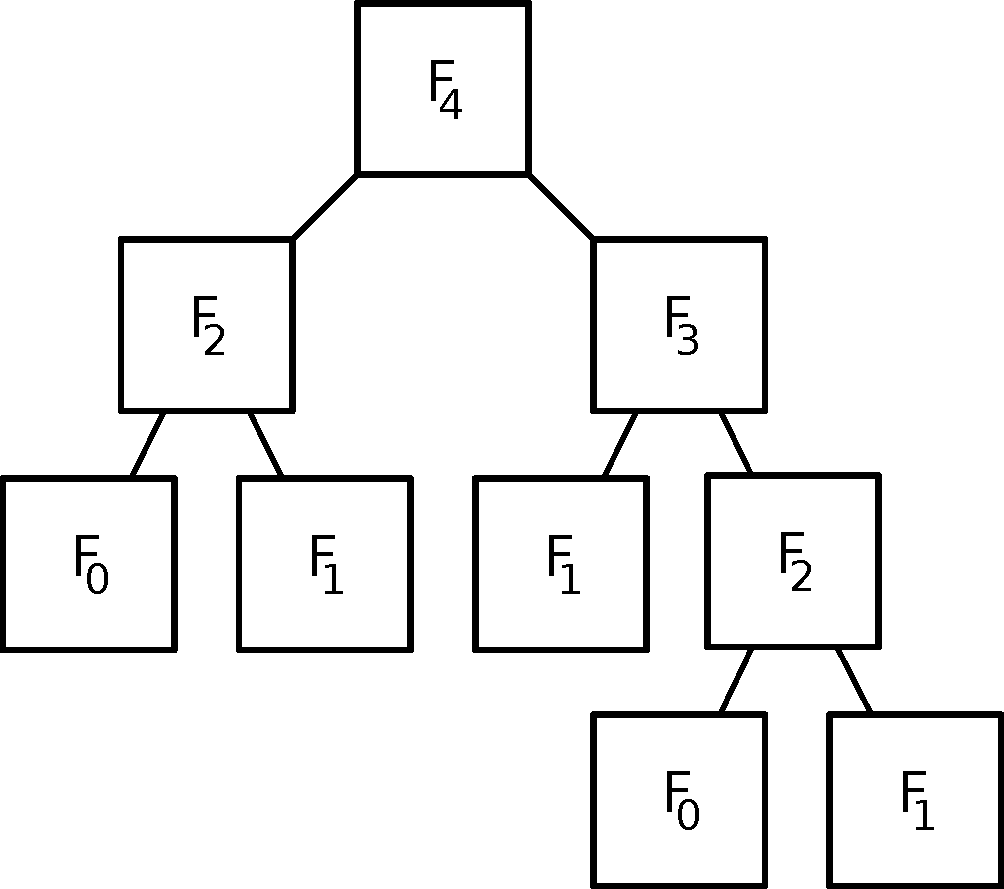
\includegraphics[width=\textwidth]{fib-block.pdf}
	
	\caption{A diagram showing the dependencies for the recursion of calculating the fourth Fibonacci number.}
	\label{fib_block}
\end{figure}

We can see the contrast between hardware and software in the determinant calculation described earlier. A software implementation, like the one listed in \ref{recursion_time} takes time but uses very little space, whereas the hardware implementation listed in \ref{recursion_space} takes almost no time but a lot of space, and the code I present is limited to $4\times4$ matrices or smaller, despite both implementing the same naive, recursive algorithm. Here we see the differences between hardware and software---hardware is inherently parallel, whereas software is inherently sequential. For the software side, consider multi-core CPUs. Writing programs that run in parallel is more difficult than single-threaded programs since care has to be taken to prevent contention and race conditions. For the hardware side, consider the CPU I presented earlier. Assuming I wanted to print the numbers from some value $n$ down to zero, I could simply have created a Verilog ``generator'', which would have generated the hardware to print all those numbers, similar to an unrolled for loop in a language like C. Thus we can see that designing hardware that runs tasks in series is more difficult than designing hardware that runs tasks in parallel, and designing software that runs tasks in parallel is more difficult than designing software that runs tasks in series.

The other advantage hardware has over software is that it can be made very specific to an application, meaning that the overhead associated with having a CPU can be removed for the specific hardware concerned. For example, a hardware Fibonacci module does not require complex instruction decoding circuitry because it only performs one operation.

One final thing to note is that---as with most things---the optimal methods are usually somewhere in the middle. For example, my matrix multiplication module performs a sequence of dot products sequentially (like a CPU), however each multiplication operation in the dot product module is performed in parallel. Likewise, as I alluded to before, many pieces of software are being optimised for our modern multicore systems, and modern CPUs support SIMD instructions, which are similar to my dot product module---the same instruction / operation (multiplication) is performed on multiple pieces of data (each pair of entries in the vectors).

\subsection{FPGA Design Flow}

Before moving on, I would like to briefly discuss the FPGA design flow, i.e.\@ how to put Verilog (or any other HDL) onto an FPGA. There are three main steps:

\begin{enumerate}
	\item Synthesis: This is the process where the HDL code is converted into a netlist. A netlist is a description of all of the logic operations (e.g.\@ logic gates, flip flops, multipliers, etc.\@), and all the connections between those logic operations. This step is mostly independent of the target FPGA.
	\item Placement and Routing (P\&R): This is where the LUTs and other features of the FPGA are all wired together according to the netlist. This generates a ``bitstream'' which is what is uploaded to the FPGA to make it reconfigure itself to do what the HDL code specified. This step is specific to the hardware that is being targeted, since it needs to know the physical layout of the FPGA to optimise which netlist logic unit should go on which hardware logic unit, and how to best connect them all.
	\item Flashing: This is where the bitstream is sent to the FPGA. The FPGA processes the bitstream, configures its LUTs and other logic units, and connects them all together via its internal switching fabric.
\end{enumerate}

Alternately, the HDL code could be synthesised to an application specific integrated circuit (ASIC), which is a non-reconfigurable silicon chip. The process is very much the same as with an FPGA (apart from flashing the bitstream) except that there is much more flexibility in P\&R process, however this involves the full integrated circuit fabrication process, making it much more time consuming and expensive.

\section{Implementation and Results}

This section can be broken into two stages: The first is about getting a basic Kalman filter working in software, and the second is about implementing a Kalman filter in hardware.

\subsection{Python Kalman Filter}
The first phase of the project was getting a simple Kalman filter working. I will start by restating two important equations for the Kalman filter. Firstly, we have how the state is updated over time
$$\mathbf{x}_k = \mathbf{F}_k \mathbf{x}_{k-1} + \mathbf{B}_k \mathbf{u}_k \,,$$
where $\mathbf{x}_k$ is the state at some time step $k$, $\mathbf{F}_k$ is the state transition model which shows how the state evolves on its own, and $\mathbf{B}_k$ is the control input model which shows how the system response when perturbed by an input $\mathbf{u}_k$.

The second equation shows how the measurements are predicted by the state
$$\mathbf{z}_k = \mathbf{H}_k \mathbf{x}_k \,,$$
where $\mathbf{z}_k$ are the measurements, and $\mathbf{H}_k$ is the matrix which maps state to measurements.

\subsubsection{Example Situation One: Position}
The first situation was the case of a simple one-dimensional cart moving backwards and forwards, with the measured quantity being position. In this case, the state is
$$\mathbf{x} = \begin{bmatrix} x \\ \dot{x} \end{bmatrix} \,,$$
where $x$ is the position. The state transition model is
$$\mathbf{F} = \begin{bmatrix} 1 & \Delta t \\ 0 & 1 \end{bmatrix} \,,$$
where $\Delta t$ is the time step. This represents position increasing by velocity multiplied by the time step. The control vector is
$$\mathbf{u}_k = \begin{bmatrix} a \\a\end{bmatrix} \,,$$
i.e.\@ the system is being perturbed by some acceleration, $a$. In this example, the acceleration will be sinusoidal. The control input model is 
$$\mathbf{B} = \begin{bmatrix} \frac{1}{2} {\Delta t}^2 \\ \Delta t \end{bmatrix} \,,$$
which just represents discrete integration of acceleration to get velocity and position. Finally, the measurement matrix is
$$\mathbf{H} = \begin{bmatrix} 1 & 0 \end{bmatrix} \,,$$
i.e.\@ we are measuring position, so $\mathbf{z}_k=x$.

In figure \ref{1d_position_fig} we can see the system handles both a fairly predictable motion as well as an unpredictable motion quite well. 

This is to be expected since we are measuring position, thus we expect the estimate of position to be fairly accurate (for obvious reasons). The estimate of velocity slowly converges to the actual velocity, however it has to re-converge after the bump. This is also expected since the bump was modelled as an impulse, which isn't a 100\% realistic scenario.

\begin{figure}[thp]
	\centering
	
	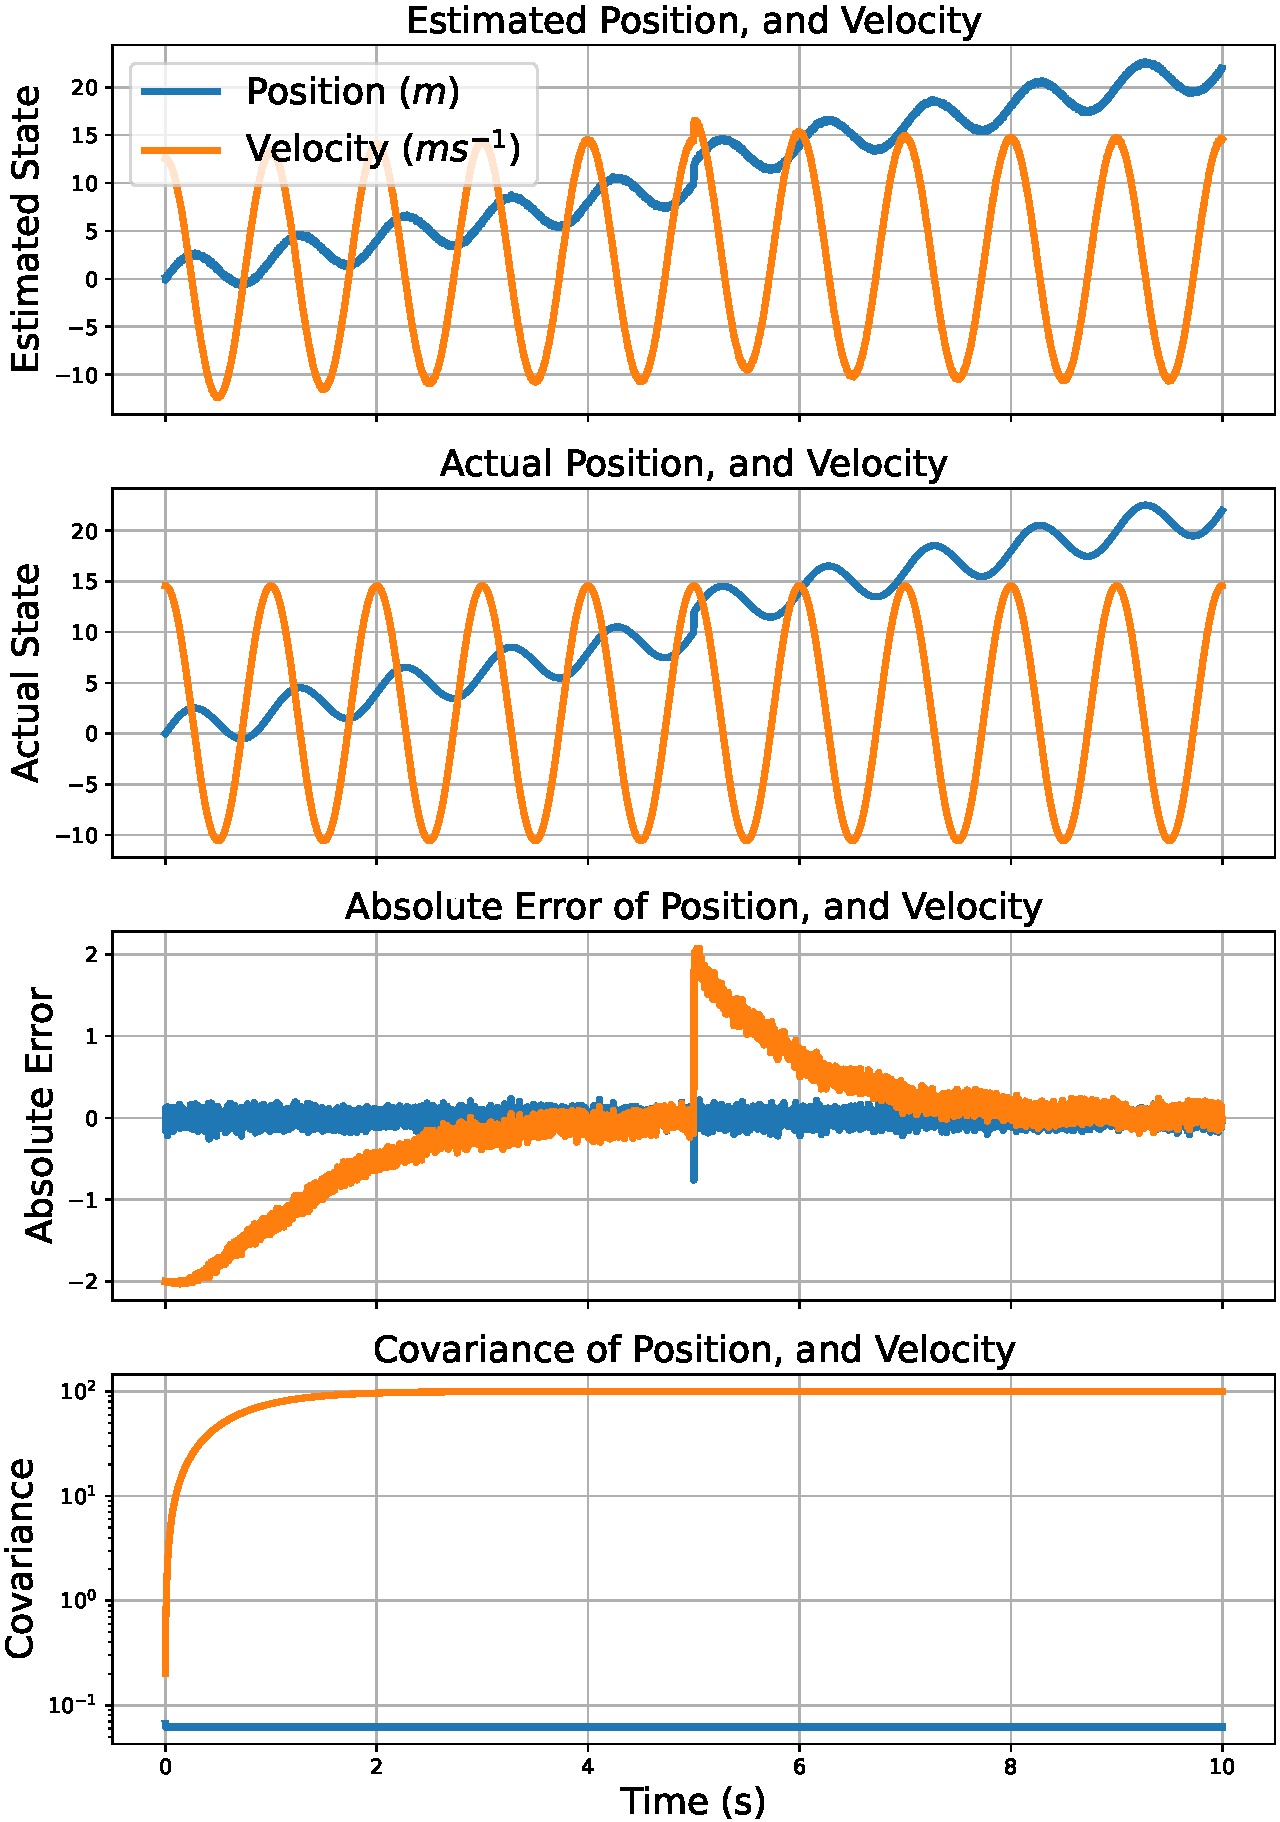
\includegraphics[width=\textwidth]{1d-position.pdf}
	
	\caption{A cart moving backwards and forwards, with a slight tendency to move in the positive direction. The cart is ``bumped'' at $t=5$, where we see the error of the velocity increase, until it settles down into a new equilibrium.}
	\label{1d_position_fig}
\end{figure}

\subsubsection{Example Situation Two: Velocity}

The next system was the same as before except the velocity was measured, and the position determined by integrating---i.e.\@ by adding the velocity multiplied by the time step to the previous position. All variables are the same as with the first situation, except that
$$\mathbf{H} = \begin{bmatrix} 0 & 1 \end{bmatrix} \,,$$
and thus we are measuring velocity, so $\mathbf{z}_k=\dot{x}$.

In this scenario, the velocity is sinusoidal, with a gradual linear increase over time. As we can see in figure \ref{1d_velocity_fig}, the model continues to perform well, with minimal error which appears to be bounded.

\begin{figure}[thp]
	\centering
	
	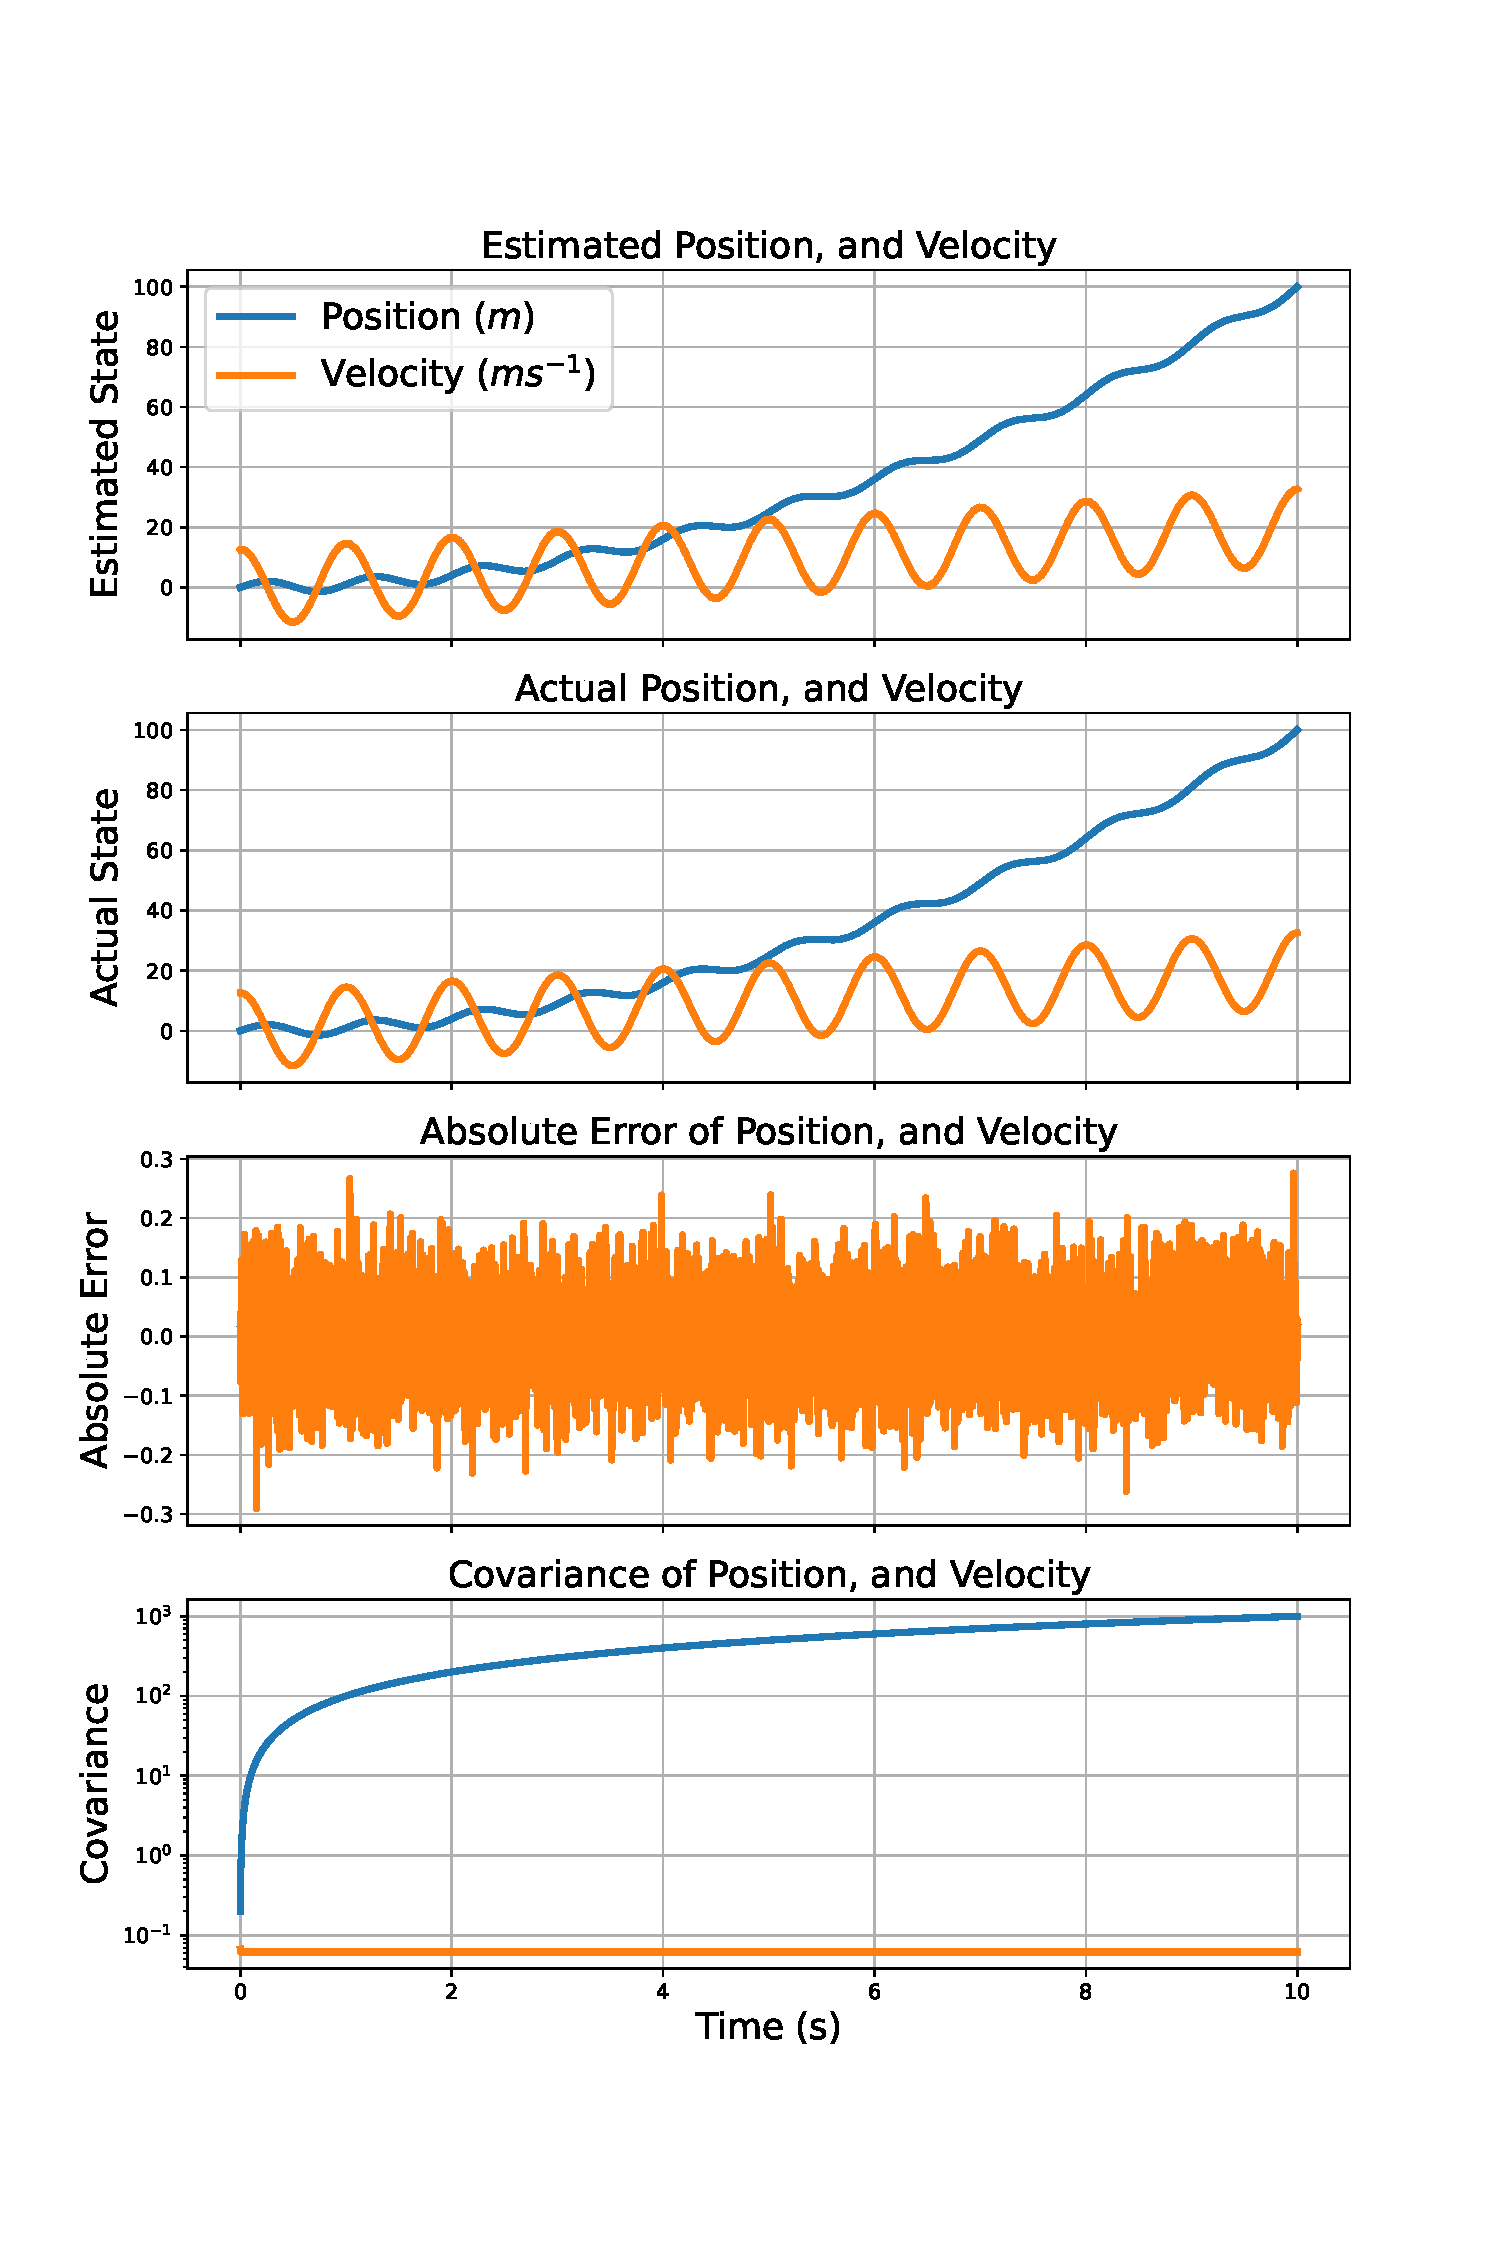
\includegraphics[width=\textwidth]{1d-velocity.pdf}
	
	\caption{Here we see the estimate of the state continue to be fairly accurate, even when faced with an unconstrained motion in the positive direction.}
	\label{1d_velocity_fig}
\end{figure}

\subsubsection{Example Situation Three: 3D Orientation}

The final scenario is that of a three-dimensional body oscillating backwards and forwards on all three axes, from $\theta=0$ to $\theta=\pi$. This time the state\footnote{I won't present the matrices and vectors since their length is unwieldy (especially given that they tend to be very sparse) and don't provide any useful information.} contains three elements (one for each axis) for each of orientation, angular velocity, and the angle between the measured orientation and some known orientation (this stands in for something like the magnetic field vector in real life). The state transition model is simply integrating angular velocity and adding it to orientation to get an updated orientation. The control input model is similar, as it just sets the angular velocity. Finally, the measurements are of angular velocity and the fake ``magnetic field''.

This also shows decent performance, which we can see in figure \ref{3d_orient_fig}. The error is low, and more importantly stays low (i.e.\@ doesn't run off to infinity).

\begin{figure}[thp]
	\centering
	
	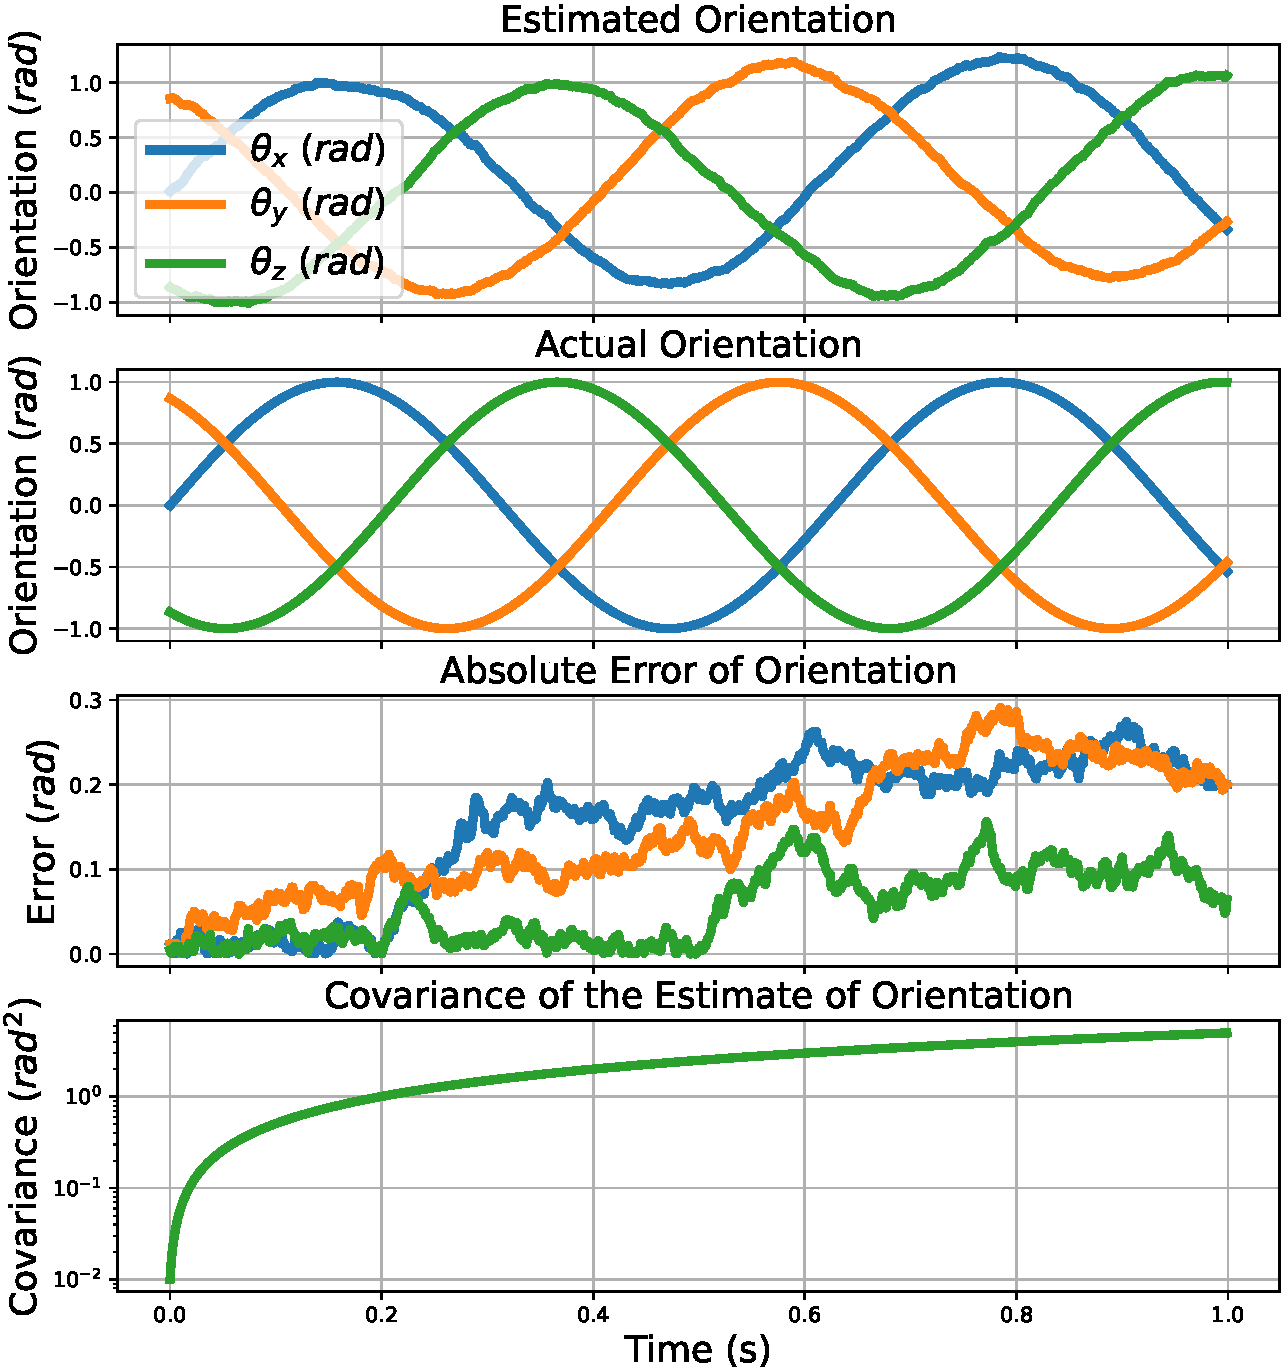
\includegraphics[width=\textwidth]{3d-orientation.pdf}
	
	\caption{A decent estimate of the orientation given noisy data. The covariance grows slowly.}
	\label{3d_orient_fig}
\end{figure}

From this we can also demonstrate how sensor and model noise affect the accuracy of the orientation estimate. For a discrete data set, the root-mean-square is defined as the square of the average of those values squared, i.e.

\newcommand{\RMS}{\ensuremath{\mathit{RMS}}} % <dme> oh, oops - you use RMS once in maths. The command is a bit of overkill then!! :-) Still, the mathit fixes the inter-letter spacing.
\begin{equation}
	x_\RMS = \sqrt{{1 \over n}(x_1^2 + x_2^2 + \dots + x_n^2)}
\end{equation}

If we run multiple iterations of the three dimensional scenario, altering the amount of noise added to the measurements and system each time, we can calculate the RMS of these error values and plot that against the magnitude added noise, as shown in figure \ref{3d_rms_fig}.

\begin{figure}[tp]
	\centering
	
	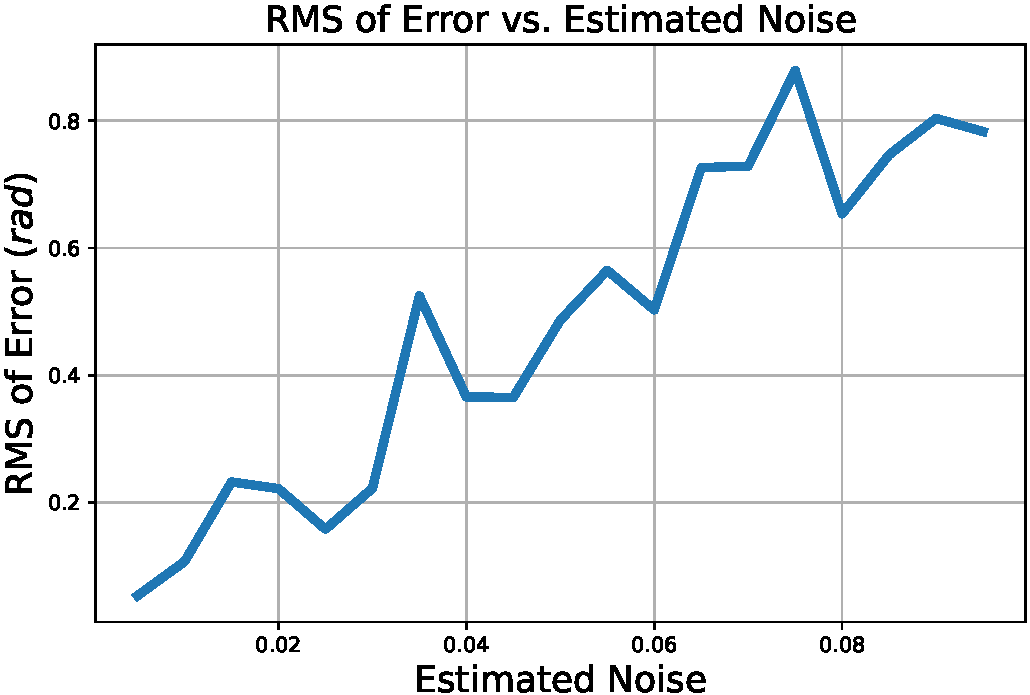
\includegraphics[width=\textwidth]{3d-rms.pdf}
	
	\caption{A plot showing the average error increasing as the amount of noise increases. The growth is approximately linear.}
	
	\label{3d_rms_fig}
\end{figure}

Here we see linear growth (with some variation)---as we make the simulated sensors more noisy the quality of the output goes down. We can see the effect of this noise in figure~\ref{3d_noise_fig}---where the noise is five times greater than in figure~\ref{3d_orient_fig}.

\begin{figure}[thp]
	\centering
	
	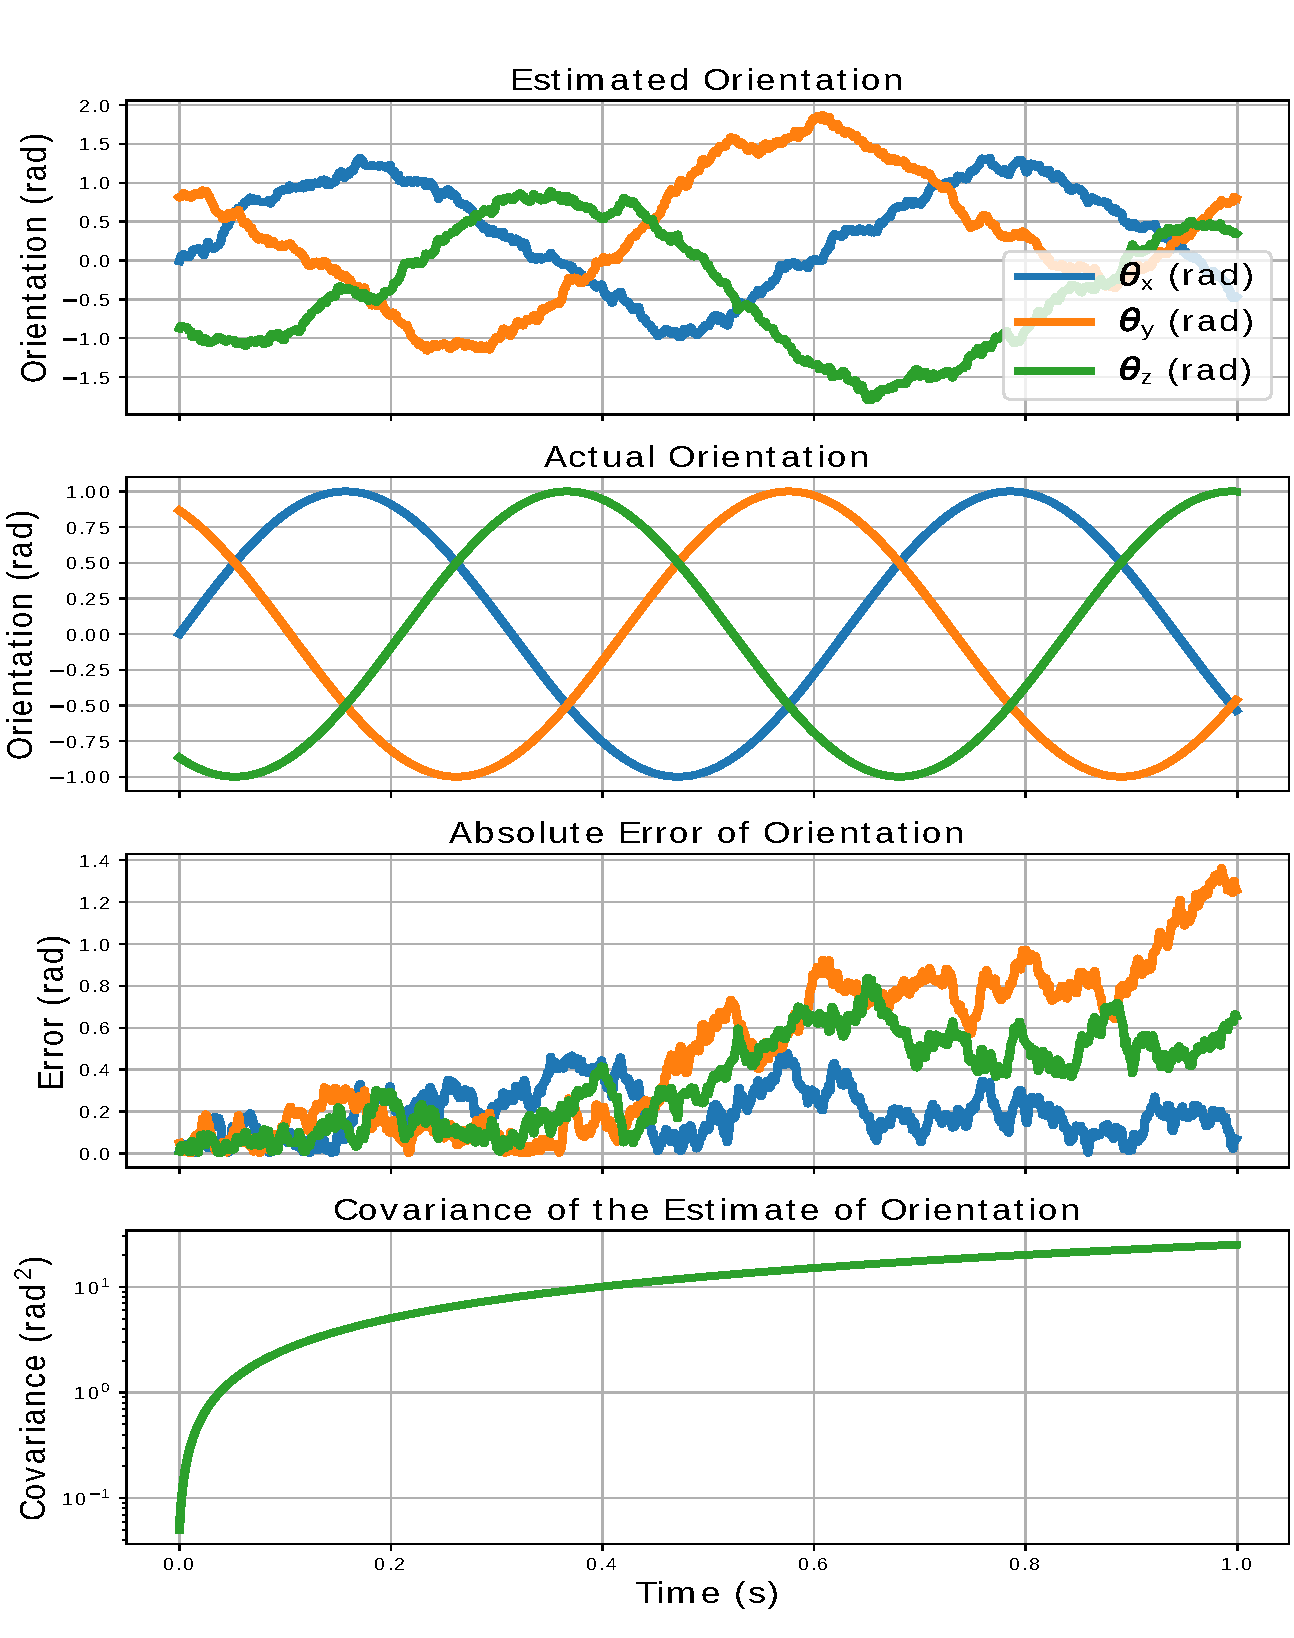
\includegraphics[width=\textwidth]{3d-orientation-noisy.pdf}
	
	\caption{The filter performing much worse---but the error is still bounded---and the shape of the periodic curves does approximately match reality.}
	\label{3d_noise_fig}
\end{figure}

\subsection{Verilog Matrix Operations}

Now that I have a few software implementations of the Kalman filter, I can move on to how I might implement it in hardware.

As can be seen in \ref{recursion_space}, the amount of Verilog code required to perform a moderately complicated mathematical operation is quite vast. The $4\times4$ code I show could be written by hand fairly easily, however this would not be possible for the $12\times12$ matrix required---even a $9\times9$ version took up 40 slides in Beamer.

The solution is to automatically generate the Verilog code in software---this is the approach I used for the code in \ref{recursion_space}. This is not a trivial task but it is significantly easier to write a few hundred lines of Python than 20 KiB of Verilog. In addition to automatically generating the Verilog code, I have also created some testbench modules and an associated Python script to automatically test that my automatically generated code is actually correct. This works by firstly generating the relevant Verilog modules and testbenches. It then runs the simulated testbenches using Icarus, and these output the test matrices and the output from the modules. Finally the script reads that output and compares it to a known correct result---the output from \lstinline|numpy| in Python. The script is able to vary both the size of the input matrices, and the width (how many bits) of the data values.

For the values, I used fixed point numbers. I chose fixed point over floating point since I am able to quantify how precise I require the input numbers to be, thus I don't need the huge range of values that are possible with floating point. Fixed point is also easier to implement, since the basic operations (addition, subtraction, multiplication, and division) are the same as with their integer counterparts, except that multiplication needs to be coupled with a right shift of the width of the decimal component, and division needs a left shift of the width of the decimal component.

\subsubsection{How the Width of Numeric Data Affects Error}

Regardless of the choice of representation for the numbers I expect both my code and the test script (i.e.\@ the results from \lstinline|numpy|) give the same result. However if the integer component is too small, then we will likely get error caused by overflow or underflow (e.g.\@ if the integer component is only 8 bits wide and we try to calculate $23 \times 57$ the result will be incorrect), and if the decimal component is too small then the precision of the result will fall, since we are unable to represent numbers with sufficient accuracy. There is no downside (in an accuracy sense) from making the numbers very large (e.g.\@ 1024 bits wide, with a 512-bit wide decimal component), however this will require more hardware resources (in the context of an FPGA, it would require more lookup tables (LUTs) and more multipliers, for example). It is a huge waste to over-provision like that, so we will want to investigate exactly how wide we need the numbers to be.

The testbench model gives the following output when the matrix values are integers between -10 and +10, and all numbers are 8 bits long (with no decimal component), for the determinant of $2\times2$ matrices. It outputs information when the result from Icarus differs from what Python's \lstinline|numpy| library expects. Here we can see the module failing occasionally due to integer overflow\footnote{Note that in each case, if we flip all the bits in the numbers labelled ``Parsed matrix determinant'' and add one, then the number will be (when interpreted as a two's compliment number) the same as the number labelled ``Icarus determinant''.} somewhere in the operation, due to the size of the numbers:
\lstinputlisting[numbers=none, backgroundcolor=\color{white}]{testbench-output-28.txt}
With 16-bit numbers, all 1000 runs for the $2\times2$ matrices succeed. For a $6\times6$ matrix, 24-bit numbers are needed. If the range of matrix values is increased to between -100 and 100 then 48 bits are required for a $6\times6$ matrix, and 16 bits are required for a simple $2\times2$ matrix.

If we now move to numbers with a decimal component (while still restricting ourselves to the determinant module), we can also determine that for a $12\times12$ matrix with numbers ranging from 0 to 10 (similar to what I would expect to see in a Kalman filter), 128-bit numbers are required, with 64 bits for the integer component, and 64 bits for the decimal component. This is shown in figures \ref{full_heat_det} and \ref{full_sfc_det}. What we can also see is that the integer width needs to be sufficient to prevent overflow, and no more, i.e.\@ there is no benefit to using larger integer components. This is in contrast to the decimal component, where we see that increasing that reduces error linearly, until about 56 bits where it starts to flatten out.

A similar pattern is visible with the matrix inverse operation (figures \ref{full_heat_inv} and \ref{full_sfc_inv}), except in that case the integer width makes even less of an impact---any integer component greater than 8 bits is sufficient. One final operation worth discussing is matrix multiplication. In figures \ref{full_heat_mul} and \ref{full_sfc_mul}, we can see that the matrix multiplication operation is much more consistent and predictable that the inverse and determinant operations. This arises primarily because calculated values are not dependant on previously calculated values, e.g.\@ for $\mathbf{AB}=\mathbf{C}$, $c_{ij}$ does not depend on any other previously calculated values in $\mathbf{C}$, meaning that there is no global error, only local error. Compare that to the LU decomposition---for the lower triangular matrix $\mathbf{L}$ values are dependant on values above them in the same column, thus numeric error can compound. In any case, we can still see that in all cases integer width only matters up until a point, whereas the accuracy falls of more slowly as the decimal width is reduced. I will also note here that the transposition operation had no error, since all it does is rearrange the data in a given matrix.

\begin{figure}[thp]
	\centering
	
	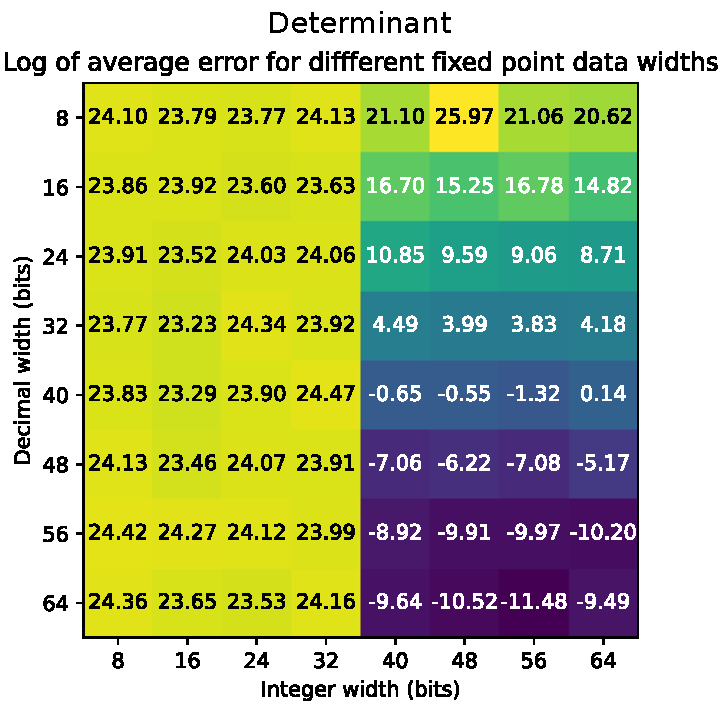
\includegraphics[width=\textwidth]{heatmap_full_det.pdf}
	
	\caption{A heat-map of the base 10 $\log$ of the average error of the determinant (when compared to the result from \lstinline|numpy|), after 10 runs for a $12 \times 12$ matrix. Darker colours (smaller numbers) are better.}
	\label{full_heat_det}
\end{figure}

\begin{figure}[thp]
	\centering
	
	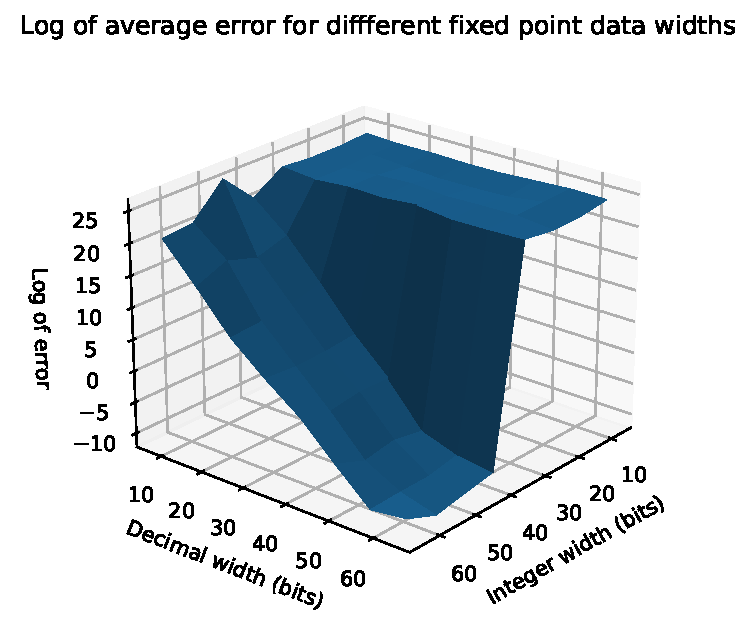
\includegraphics[width=\textwidth]{sfc_plot_full_det.pdf}
	
	\caption{The same plot as in figure \ref{full_heat_det}, but as a 3D surface plot as opposed to a heat-map. The steep gradient at around a 40-bit wide integer component is very visible here. Lower is better.}
	\label{full_sfc_det}
\end{figure}

\begin{figure}[thp]
	\centering
	
	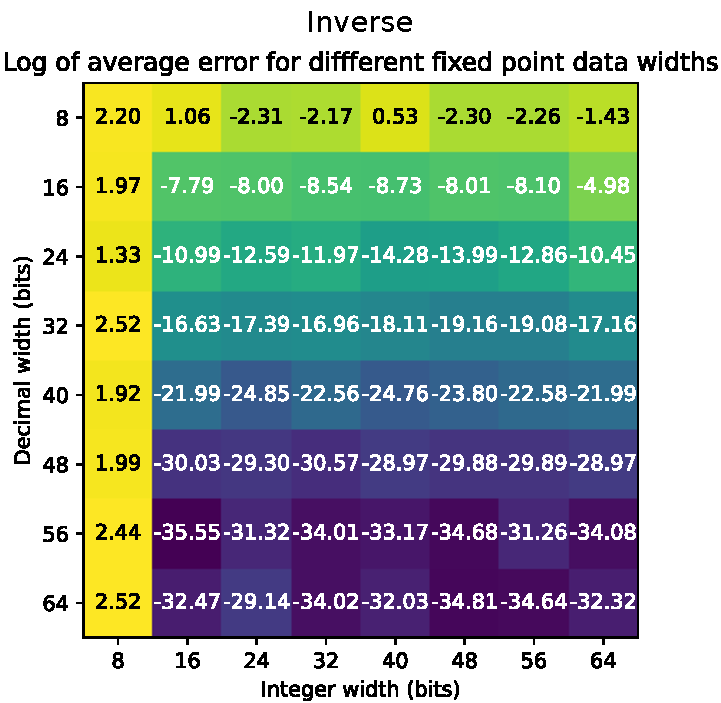
\includegraphics[width=\textwidth]{heatmap_full_inv.pdf}
	
	\caption{Another heat-map, this time for the inverse. The drop-off for sufficiently wide integer components occurs a lot sooner here. Darker colours (smaller numbers) are better.}
	\label{full_heat_inv}
\end{figure}

\begin{figure}[thp]
	\centering
	
	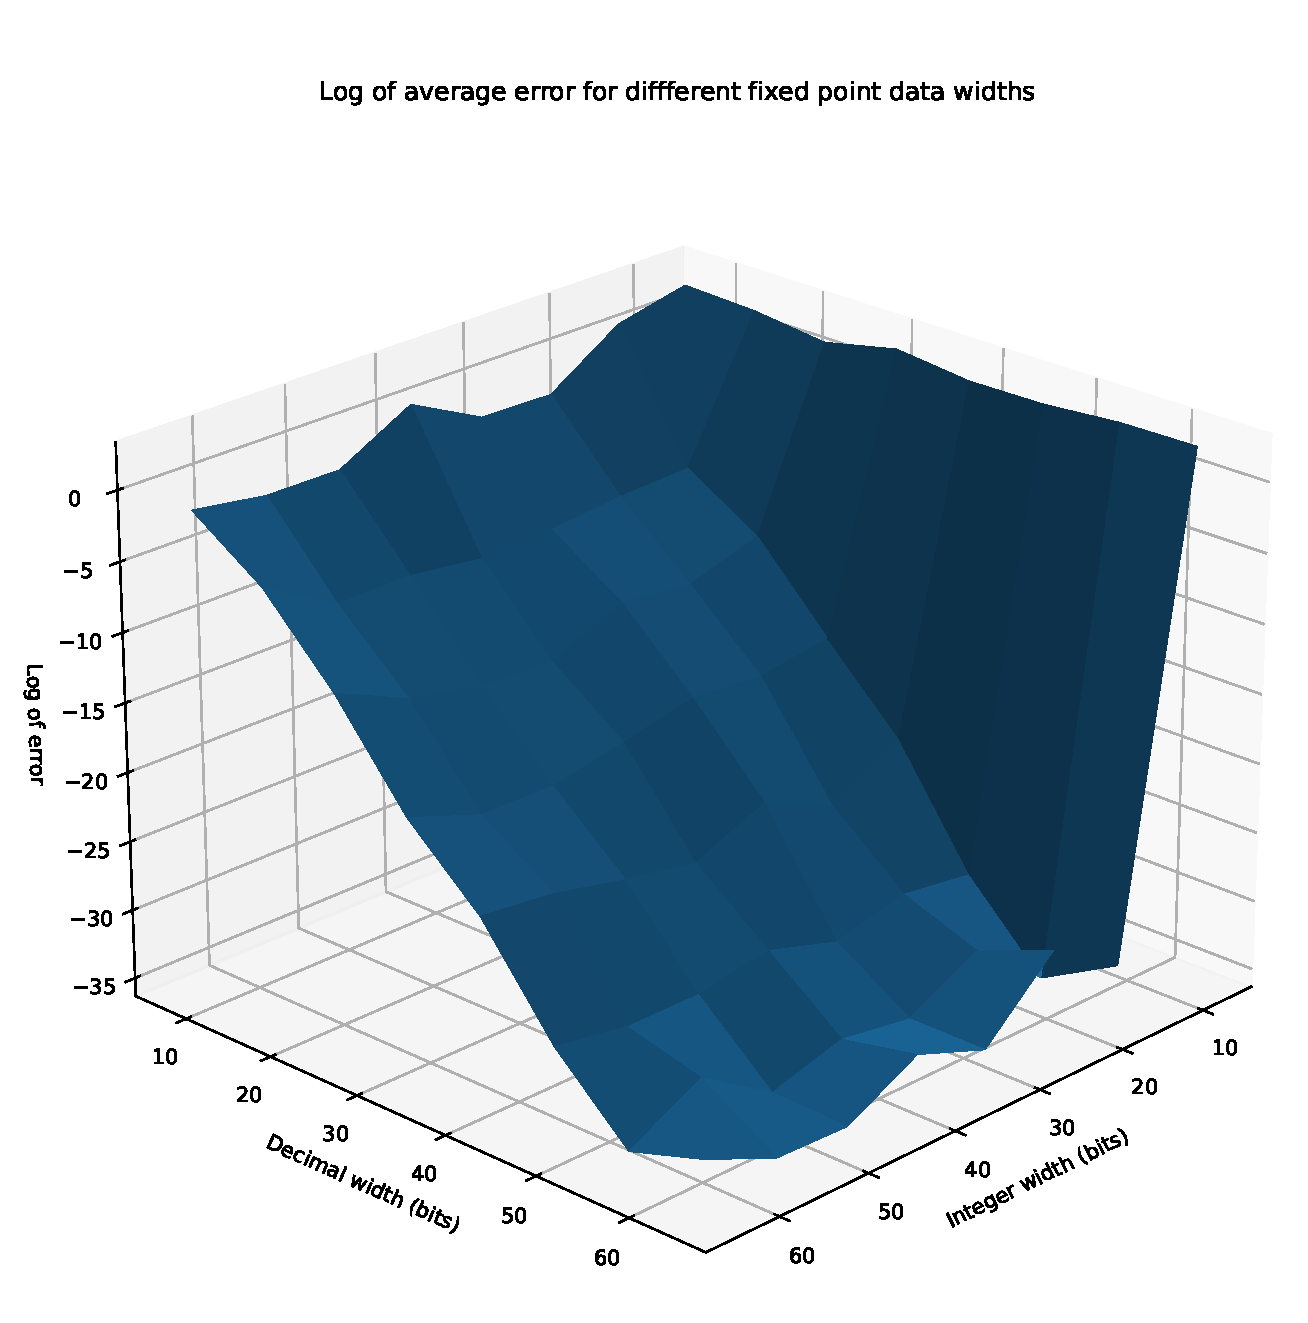
\includegraphics[width=\textwidth]{sfc_plot_full_inv.pdf}
	
	\caption{Another surface plot, this time for the inverse. Lower is better.}
	\label{full_sfc_inv}
\end{figure}

\begin{figure}[thp]
	\centering
	
	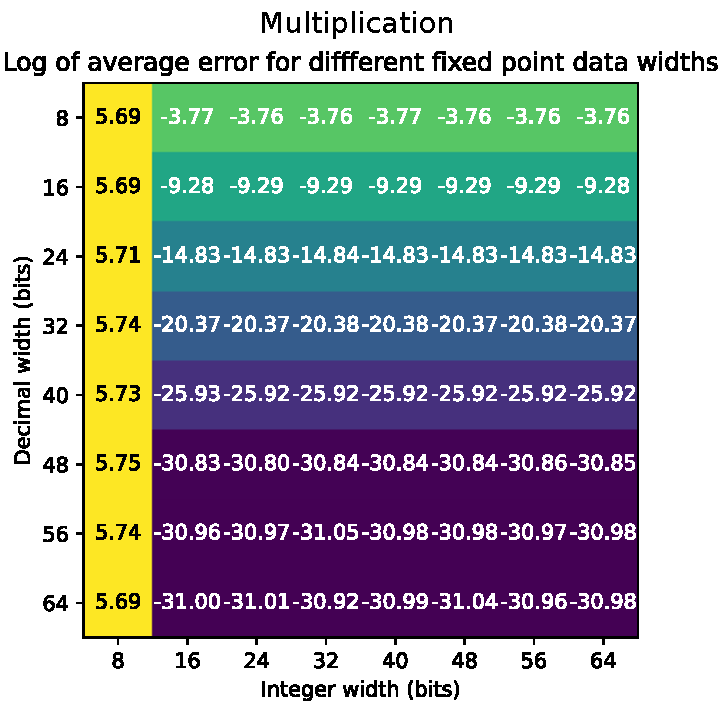
\includegraphics[width=\textwidth]{heatmap_full_mul.pdf}
	
	\caption{Another heat-map, this time for matrix multiplication. The much greater consistency is very visible here. Darker colours (smaller numbers) are better.}
	\label{full_heat_mul}
\end{figure}

\begin{figure}[thp]
	\centering
	
	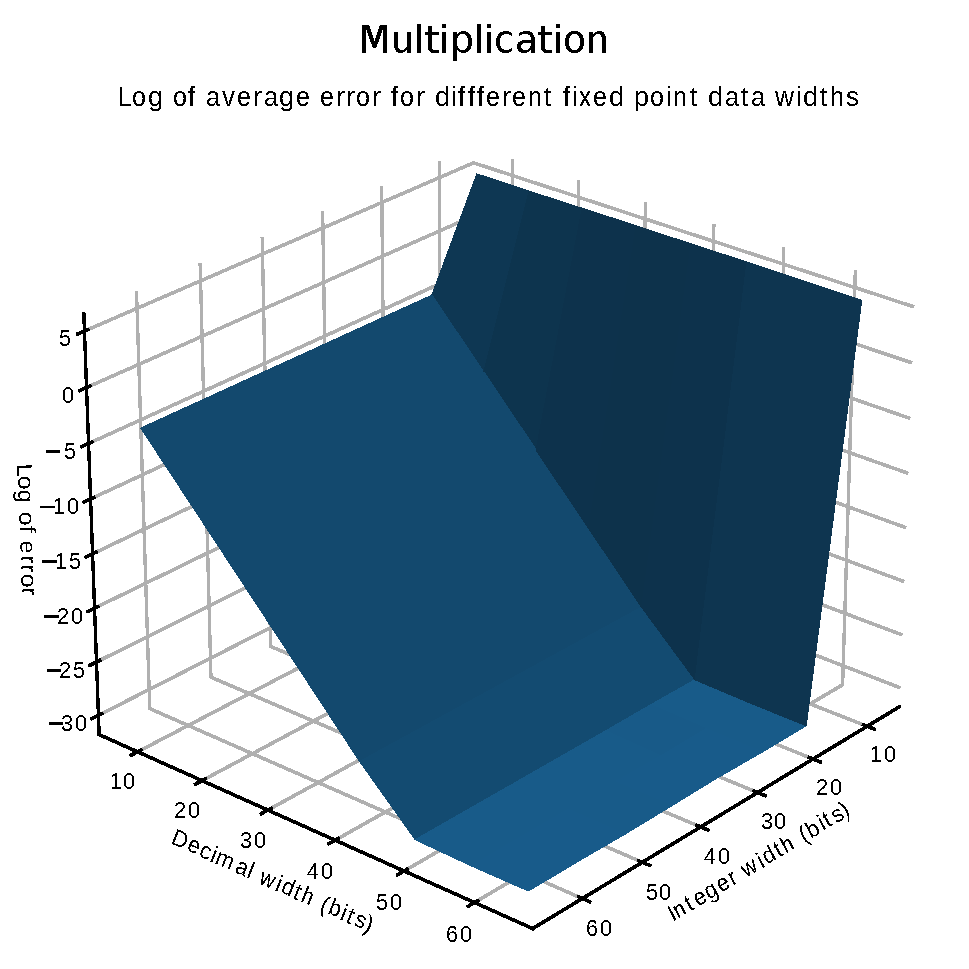
\includegraphics[width=\textwidth]{sfc_plot_full_mul.pdf}
	
	\caption{Another surface plot, this time for matrix multiplication. The consistency of the matrix multiplication operation is very visible here---it almost looks like an empty swimming pool. Lower is better.}
	\label{full_sfc_mul}
\end{figure}

\subsubsection{How the Choice of Algorithms Affects Performance}

My first implementation of the matrix operations was using the naive algorithms, as described in section \ref{naive}. This implementation worked, however when it came to simulating the Verilog, both the determinant, and even more so the inverse took a very long time for the $12 \times 12$ case. I had estimated that simulating the $12 \times 12$ inverse would take about a whole day, and also be far too time consuming to implement in practice. As a result of this, I turned to the LU decomposition, as discussed in section \ref{lu}. Initially, I only converted the determinant operation to use the LU decomposition--- i.e.\@ the inverse operation was the ``half-naive'' inverse. Despite the inverse only being half optimised, it still made a huge difference: The simulation time dropped to 10 minutes---and the predicted performance wasn't too bad---about 2.5 million clock cycles to complete an operation. On a 100 MHz FPGA this could do 40 operations per second. Since there is only one inverse per Kalman Filter cycle, and the inverse operation takes the longest by far of all of the operations, I would expect to be able to run about 40 Kalman filter cycles per second, which would be sufficient for real time operation. This is still not ideal however, so I tried again with the fully optimised inverse. Again, there was a huge speed up in simulation time---from 10 minutes to one second. Compared with the fully naive implementation this represents an 86,400$\times$ speed-up. The actual performance improved hugely as well, down to only 58,674 clock cycles. At 100 MHz this represents 1700 inverses per second. Since the inverse still represents the longest operation (58,674 cycles versus 145 clock cycles for $12\times12$ multiplication), then this would represent 1700 Kalman filter cycles per second, i.e.\@ less than one milliseconds per filter cycle. Assuming, hypothetically, that a chip made from this design could run at the speed of a CPU, e.g.\@ 3.6 GHz\footnote{This assumption is based on running \lstinline|grep -i mhz /proc/cpuinfo| and looking for the biggest number.}, this would represent 61,200 filter cycles per second, or a filter cycle every 16 microseconds.

\subsubsection{Synthesis and Implementation}

Due to time constraints I was not in a position to put a final bitstream on an FPGA, however I was able to synthesize it, and place and route it, based on the target device being a Xilinx Artix-7 XC7A100TCSG324, shown in figure~\ref{tim_xilinx}.

\begin{figure}[thp]
	\centering
	
	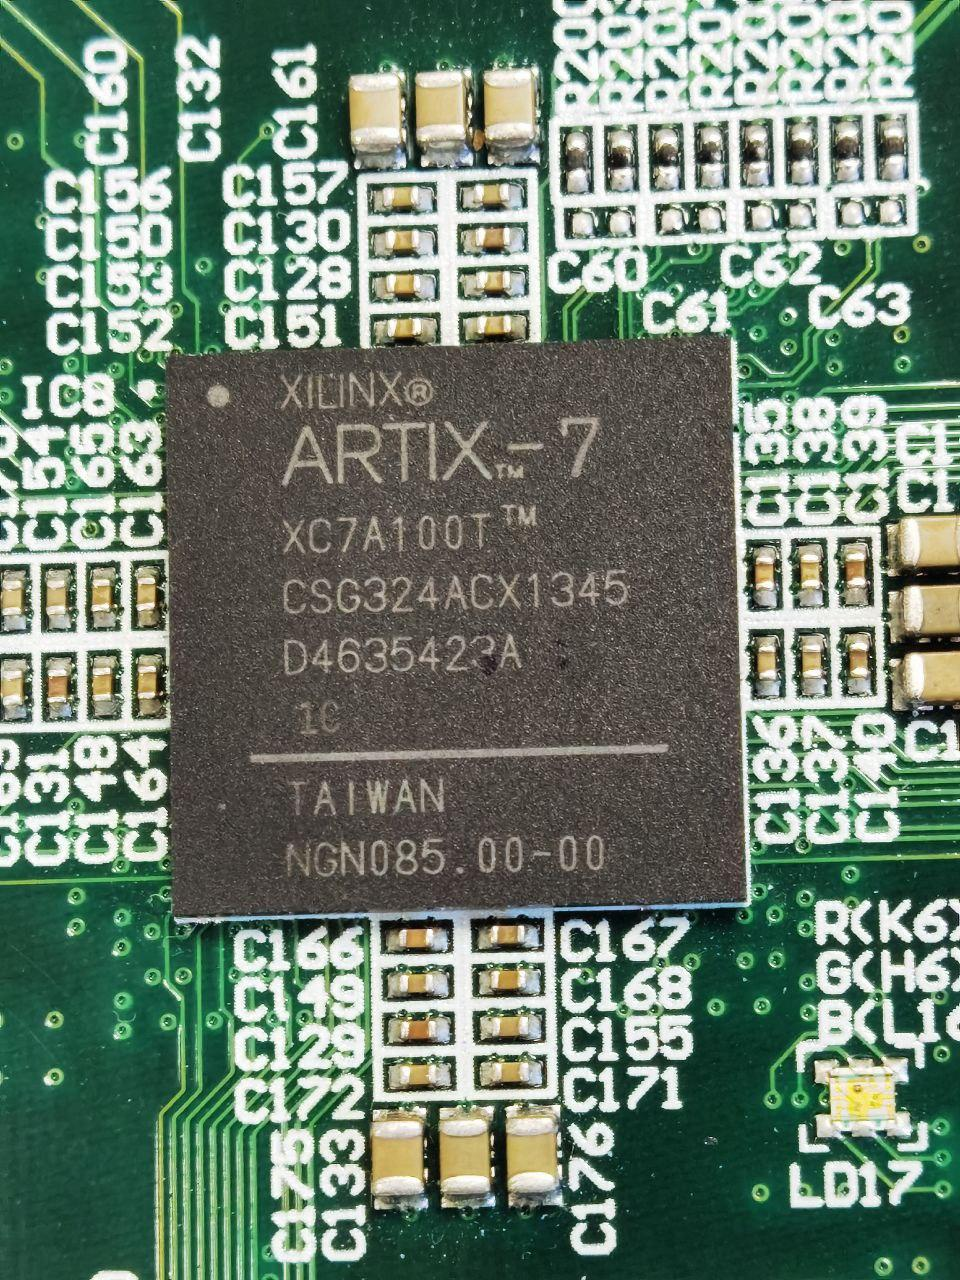
\includegraphics[width=\textwidth]{tim_xilinx.jpg}
	
	\caption{The sort of FPGA I would target for this project.}
	\label{tim_xilinx}
\end{figure}

This FPGA has 63,400 LUTs, and 240 DSPs (multiplier units), which should be sufficient for the purposes of this project. A development board with this FPGA on it costs around \$129.00 USD, which is entirely reasonable. Of course this would not be acceptable for a chip to be included in a phone, however FPGAs are much more expensive than non-configurable hardware, so I would expect the per-unit cost for a fabricated chip that fit on the XC7A100TCSG324 to cost less than one dollar.

Because the DSPs on the FPGA I am using only support multiplication of 25-bit and 18-bit numbers, it was not sufficient for even the $4\times4$ modules (with semi--naive inverse) with 128-bit wide numbers, as it required 74,989 LUTs and 1008 DSPs. As a workaround, I artificially limited the width of the numbers going into the multiplier units to only be 16 bits wide (while keeping the correct widths elsewhere). This reduced the requirements to 38,027 LUTs and 5 DSPs, which would fit on the Artix-7 FPGA I was targeting. By using the fully LU based inverse module, this was further reduced to 24,569 LUTs and 2 DSPs.

In order to show how increasing the size of the matrices increases the resource usage, I synthesized only the inverse module, with 16-bit wide numbers. The results are in the table below:

\begin{center}
	\begin{tabular}{ c | c c }
		Size & LUTs & DSPs \\ 
		\hline
		$4\times4$ & 3019 & 2 \\  
		$8\times8$ & 10,330 & 2 \\
		$12\times12$ & 22,426 & 2
	\end{tabular}
\end{center}

This indicates that with some optimisation, it would be possible to fit this on such an FPGA. This would require ensuring that addition was constrained to run on the DSPs, and not via adders cobbled together from LUTs, since this is likely the culprit for the high LUT usage and low DSP usage. This would free up enough LUTs to expand to the full 128-bit wide numbers. In order to get around the 25-bit by 18-bit limit, I would likely use the Karatsuba algorithm \cite{karatsuba} to break the multiplication into chunks.

\section{Future Work}

Certain specific tasks that could be done in future include:

\begin{itemize}
	\item Further optimise the mathematics to reduce LUT count.
	\item Optimise the multiplication operator to allow it to use DSPs efficiently for numbers of any width.
	\item Piece together a Kalman filter from the matrix mathematics modules, and quantify the error for the whole filter. This could then be interfaced with sensors to provide state estimation.
	\item Flash a bitstream to an FPGA.
\end{itemize}

\section{Conclusion}

The project started out as an attempt to implement a Kalman filter in Verilog, but pivoted to take more of a focus on the matrix operations that make up the Kalman filter. In particular, I ended up focusing on optimising the matrix mathematics (still with the Kalman filter in mind, since I performed the tests on a $12 \times 12$ matrix), in terms of the precision of the representation of the numbers, and in terms of how optimal the algorithms that I was using are. Through this process I was able to show how integer width needs only be sufficient, whereas increasing the decimal width provides much greater, but more gradual, improvements. I was also able to show how using the correct algorithms results in a huge speed up in performance, by looking at the naive inverse and determinate, versus the LU decomposition based inverse and determinant, and also using a semi-naive inverse based on the naive inverse but the optimised LU based determinant.

While I was not able to get the code flashed to an FPGA, I was able to get it to synthesize and be placed and routed in such a way that it would fit on the target FPGA.

\printbibliography

% Activate the appendix
% from now on sections are numerated with capital letters
\appendix

\renewcommand{\thesection}{Appendix \Alph{section}}

\section{Basic CPU in Verilog}
\label{verilog_cpu}

\lstinputlisting[language=Verilog]{cpu-include.v}

\section{Example of Recursion in Time}
\label{recursion_time}

\lstinputlisting[language=Python]{recursion-time.py}

\section{Example of Recursion in Space}
\label{recursion_space}

\lstinputlisting[language=Verilog]{recursion-space.v}

\end{document}